\chapter{Metrik, Expansion und eine erste Kosmologie}

Am Ende der vorangegangenen Vorlesung hatten wir eine lorentzinvariante Wellengleichung erreicht und wollten die Maxwell-Gleichungen in Raumzeitform schreiben. Bevor wir uns nun der Gravitation zuwenden, liefert eine Frage aus dem Publikum einen nützlichen Hinweis: Wie viel einer physikalischen Theorie lässt sich allein durch Symmetrie bestimmen? Die Antwort ist eindeutig: sehr viel, aber nicht alles. Die Lorentzinvarianz schränkt die möglichen Gesetze stark ein. Sie ersetzt weder die übrigen physikalischen Annahmen noch das Experiment.

\section{Was Symmetrie nicht festlegt}

\begin{classroomqa}
\audiencequestion{Folgen die Maxwell-Gleichungen allein aus der Relativität, wenn bekannt ist, dass sich elektrische und magnetische Felder gemeinsam unter Lorentz-Transformationen transformieren?}
\lecturerresponse{Nein. Die Relativität schränkt die Form der Gleichungen ein. Zu ihrer Aufstellung braucht man jedoch auch ihre Linearität, die niedrige Ordnung ihrer Ableitungen, das Transformationsverhalten der Felder und experimentelle Informationen. Ohne diese zusätzlichen Voraussetzungen wären weiterhin viele lorentzkovariante Feldgleichungen möglich.}
\end{classroomqa}

Die wichtigste dieser zusätzlichen Voraussetzungen für die einleitende Diskussion ist die Linearität. Ist \(A(x,t)\) eine Lösung einer linearen Feldgleichung, dann ist für jede Konstante \(\lambda\) auch \(\lambda A(x,t)\) eine Lösung. Sind \(A\) und \(B\) Lösungen, dann ist auch \begin{equation}
  C(x,t)=A(x,t)+B(x,t).
  \label{eq:superposition}
\end{equation} eine Lösung.
Dies ist das Superpositionsprinzip. Zwei quellenfreie elektromagnetische Wellen können einander durchdringen und unverändert wieder auseinanderlaufen. Sie stoßen nicht direkt zusammen wie materielle Körper. Indirekt können sie über geladene Materie wechselwirken: Jede Welle bewegt die Ladungen, und die bewegten Ladungen strahlen ihrerseits. Die Feldgleichungen im Vakuum sind jedoch linear.

\begin{figure}[H]
\centering
\includegraphics[width=0.64\textwidth]{lecture_08_figure_01.png}
\caption{Zwei Wellenprofile an der Tafel während der Diskussion des Superpositionsprinzips. Ihre Summe ist wieder eine zulässige quellenfreie Welle.}
\lectureframe{00:05:30}
\end{figure}

Am harmonischen Oszillator wird die Rechnung anschaulich. Es gelte \begin{equation}
  m\ddot x=-kx.
  \label{eq:linear-oscillator}
\end{equation}. Wenn \(x_1\) und \(x_2\) Lösungen von \eqref{eq:linear-oscillator} sind, dann gilt \begin{equation}
  m(\ddot x_1+\ddot x_2)
  =-k(x_1+x_2),
\end{equation}, also ist \(x_1+x_2\) eine Lösung. Ergänzt man jedoch einen nichtlinearen Term, \begin{equation}
  m\ddot x=-kx+p x^2,
  \label{eq:nonlinear-oscillator}
\end{equation}, dann ist die Summe keine Lösung mehr:
\begin{equation}
  (x_1+x_2)^2=x_1^2+x_2^2+2x_1x_2.
\end{equation}
Der Kreuzterm \(2x_1x_2\) hat in den beiden einzelnen Gleichungen kein Gegenstück. Die beiden Bewegungen beeinflussen einander nun.

\begin{figure}[H]
\centering
\includegraphics[width=0.73\textwidth]{lecture_08_figure_02.png}
\caption{Vergleich der einzelnen Oszillatorgleichungen mit der Gleichung für ihre Summe. Der quadratische Term macht den zusätzlichen Kreuzterm sichtbar, der die Superposition verletzt.}
\lectureframe{00:10:10}
\end{figure}

Dieses Beispiel verdeutlicht den methodischen Grundsatz, der für die gesamte Diskussion der Kosmologie gilt. Symmetrie legt fest, welche Größen sich kombinieren lassen und welche Gleichungen zulässig sind. Die Dynamik und die Beobachtung zeigen, welche der zulässigen Gleichungen die Natur verwirklicht.

\section{Das Intervall als Geometrie}

Wir wenden uns nun vom Elektromagnetismus ab und nehmen einen kurzen Weg in die allgemeine Relativitätstheorie und Kosmologie. Ausgangspunkt ist das Intervall zwischen benachbarten Ereignissen. Ein Ereignis werde durch die vier Koordinaten \(x^\mu\) bezeichnet, ein benachbartes durch \(x^\mu+dx^\mu\). In inertialen kartesischen Koordinaten gilt mit \(c=1\) und der Vorzeichenkonvention \((+,-,-,-)\):
\begin{equation}
  d\tau^2
  =dt^2-dx^2-dy^2-dz^2
  =dx^\mu dx_\mu
  =\eta_{\mu\nu}\,dx^\mu dx^\nu.
  \label{eq:minkowski-interval}
\end{equation}
Invariant ist die Größe \(d\tau^2\), nicht eine einzelne Koordinatendifferenz. Lorentz-Transformationen verändern \(dt,dx,dy,dz\), lassen aber diese quadratische Kombination unverändert. Die spezielle Relativitätstheorie lässt sich daher als Geometrie der Minkowski-Raumzeit auffassen.

\begin{figure}[H]
\centering
\includegraphics[width=0.72\textwidth]{lecture_08_figure_03.png}
\caption{Das Minkowski-Intervall nacheinander in Komponenten-, Indexkontraktions- und Metriktensorschreibweise.}
\lectureframe{00:14:50}
\end{figure}

Die einfache Form von \eqref{eq:minkowski-interval} hängt von den Koordinaten ab. Selbst eine flache Ebene kann ungewohnte Koeffizienten erhalten, wenn wir sie ungeschickt parametrisieren. Die Koordinate \(x\) sei in Zentimetern angegeben, \(y\) dagegen in Metern. Für eine physikalische Verschiebung gilt:
\begin{equation}
  ds^2=dx^2+\left(\frac{dy}{100}\right)^2
      =dx^2+10^{-4}dy^2.
  \label{eq:mixed-units}
\end{equation}
Der Faktor \(10^{-4}\) hat nichts mit Krümmung zu tun. Er dient lediglich der Umrechnung zwischen Einheiten.

\begin{figure}[H]
\centering
\includegraphics[width=0.59\textwidth]{lecture_08_figure_04.png}
\caption{Eine flache Ebene, beschrieben mit Zentimetern auf der einen und Metern auf der anderen Achse. Die unterschiedlichen Metrikkoeffizienten geben Einheiten wieder, keine Krümmung.}
\lectureframe{00:20:10}
\end{figure}

Schiefwinklige Koordinaten bringen einen gemischten Term mit sich. In zwei Dimensionen lässt sich die allgemeinste lokale quadratische Form schreiben als
\begin{align}
  ds^2
  &=a_{11}\,dx^2+a_{12}\,dx\,dy\notag\\
  &\quad+a_{21}\,dy\,dx+a_{22}\,dy^2,
  \qquad a_{12}=a_{21}.
  \label{eq:quadratic-form}
\end{align}
Da gewöhnliche Differentiale vertauschbar sind, \(dx\,dy=dy\,dx\), trägt nur der symmetrische Anteil der Koeffizientenmatrix bei. Wir fassen die Koeffizienten in der Matrix zusammen:
\begin{equation}
  g=
  \begin{pmatrix}
    a_{11} & a_{12}\\
    a_{21} & a_{22}
  \end{pmatrix}.
  \label{eq:metric-matrix}
\end{equation}
Diese Matrix ist die \emph{Metrik}. Sie gibt lokal an, wie Koordinatendifferenzen in physikalische Intervalle umgerechnet werden.

\begin{figure}[H]
\centering
\includegraphics[width=0.71\textwidth]{lecture_08_figure_05.png}
\caption{Die quadratische Differentialform und ihre symmetrische \(2\times2\) Koeffizientenmatrix, genau in dem Moment, in dem die Matrix als Metrik identifiziert wird.}
\lectureframe{00:24:07}
\end{figure}

Bei gleichmäßigen rechteckigen oder schiefwinkligen Gittern sind die Koeffizienten konstant. Sind die Koordinatenlinien gekrümmt oder rücken sie näher zusammen beziehungsweise weiter auseinander, werden die Koeffizienten ortsabhängig, auch wenn die zugrunde liegende Fläche flach bleibt. Die allgemeine Raumzeitnotation lautet:
\begin{equation}
  ds^2=g_{\mu\nu}(x)\,dx^\mu dx^\nu.
  \label{eq:general-metric}
\end{equation}

\begin{figure}[H]
\centering
\includegraphics[width=0.66\textwidth]{lecture_08_figure_06.png}
\caption{Die allgemeine ortsabhängige Metrik, nachdem zugelassen wurde, dass sich das Koordinatengitter von Punkt zu Punkt ändert.}
\lectureframe{00:28:10}
\end{figure}

Kennt man \(g_{\mu\nu}\) in einem festgelegten Koordinatensystem, sind damit lokale Abstände, Zeiten und Winkel und somit die Geometrie bestimmt. Die Umkehrung ist nicht eindeutig: Eine Geometrie hat unendlich viele Koordinatenbeschreibungen und damit unendlich viele Koeffizientenfelder, die durch Koordinatentransformationen miteinander verknüpft sind.

\section{Koordinatenkomplexität und intrinsische Krümmung}

Nun müssen wir eine komplizierte Metrik von einem gekrümmten Raum unterscheiden. Rollt man ein Blatt Papier ohne es zu dehnen zu einem Zylinder, ändert sich sein Aussehen im Raum, doch alle Abstände auf dem Blatt bleiben gleich. Ein Wesen, das auf das Papier beschränkt ist, kann die Biegung durch keine intrinsische Messung feststellen. Das ist extrinsische Biegung und nicht die hier gemeinte Krümmung.

Bei einer Halbkugel ist es anders. Sie lässt sich nicht ohne Dehnen, Reißen oder Stauchen flach ausbreiten. Eine flache Karte der Erde muss entweder Abstände, Flächen, Winkel oder eine Kombination davon verzerren. Dieses Hindernis ist intrinsisch und lässt sich feststellen, ohne in eine umgebende Dimension zu blicken.

Polarkoordinaten liefern das unverzichtbare flache Gegenbeispiel. Auf einer Ebene hat eine infinitesimale radiale Verschiebung die Länge \(dr\), während eine Winkelverschiebung \(d\theta\) im Abstand \(r\) die Länge \(r\,d\theta\) hat. Somit gilt:
\begin{equation}
  ds^2=dr^2+r^2d\theta^2,
  \qquad
  g_{\text{polar}}=
  \begin{pmatrix}
    1&0\\
    0&r^2
  \end{pmatrix}.
  \label{eq:polar-metric}
\end{equation}
Der Koeffizient \(r^2\) variiert über die Ebene, obwohl diese flach ist. Die Koordinatentransformation
\begin{equation}
  x=r\cos\theta,\qquad y=r\sin\theta
\end{equation}
führt zur konstanten Metrik \(ds^2=dx^2+dy^2\) zurück.

\begin{figure}[H]
\centering
\includegraphics[width=0.70\textwidth]{lecture_08_figure_07.png}
\caption{Die Metrik in Polarkoordinaten und ihre Rückführung auf die kartesische Metrik. Die ortsabhängige Matrix links beschreibt weiterhin eine flache Ebene.}
\lectureframe{00:39:20}
\end{figure}

\begin{classroomqa}
\audiencequestion{Muss die Winkelstrecke in Polarkoordinaten einen Sinus enthalten?}
\lecturerresponse{Nein, nicht in der Ebene. Dort ist die Bogenlänge \(r\,d\theta\). Auf der Kugel tritt ein Sinus auf, denn ein Breitenkreis hat den Radius \(R\sin\theta\).}
\end{classroomqa}

Wir betrachten eine Kugel mit Radius \(R\). Der Polarwinkel \(\theta\) werde vom Nordpol aus gemessen, der Azimutwinkel sei \(\phi\). Ein Schritt entlang eines Meridians hat die Länge \(R\,d\theta\). Beim Polarwinkel \(\theta\) hat der Breitenkreis den Radius \(R\sin\theta\), daher hat ein Schritt in Azimutrichtung die Länge \(R\sin\theta\,d\phi\). Nach dem Satz des Pythagoras gilt lokal:
\begin{align}
  ds^2
  &=R^2\left(d\theta^2+\sin^2\theta\,d\phi^2\right),
  \label{eq:sphere-metric}\\
  g_{\text{sphere}}=
  &\begin{pmatrix}
    R^2&0\\
    0&R^2\sin^2\theta
  \end{pmatrix}.
\end{align}

\begin{figure}[H]
\centering
\includegraphics[width=0.72\textwidth]{lecture_08_figure_08.png}
\caption{Die Kugel, ihr Winkellängenelement und die zugehörige Metrikmatrix. Der Faktor \(\sin^2\theta\) bildet ab, dass die Breitenkreise zum Pol hin kleiner werden.}
\lectureframe{00:45:15}
\end{figure}

\begin{figure}[H]
\centering
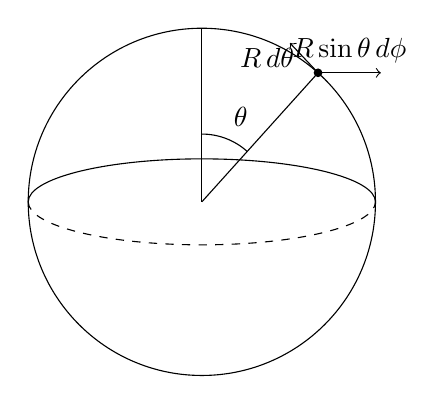
\begin{tikzpicture}[scale=1.05]
  \draw (0,0) circle (2.1);
  \draw[dashed] (-2.1,0) arc (180:360:2.1 and 0.52);
  \draw (2.1,0) arc (0:180:2.1 and 0.52);
  \coordinate (P) at (48:2.1);
  \fill (P) circle (1.5pt);
  \draw (0,0) -- (0,2.1);
  \draw (0,0) -- (P);
  \draw (0,0.82) arc (90:48:0.82);
  \node at (0.47,1.03) {\(\theta\)};
  \draw[->] (P) -- ++(-0.34,0.36)
    node[midway,left] {\(R\,d\theta\)};
  \draw[->] (P) -- ++(0.76,0)
    node[midway,above] {\(R\sin\theta\,d\phi\)};
\end{tikzpicture}
\caption{Saubere Rekonstruktion der lokalen Differentialstrecken, aus denen \eqref{eq:sphere-metric} folgt.}
\end{figure}

Keine globale Koordinatentransformation führt \eqref{eq:sphere-metric} in eine konstante euklidische Matrix über. Ein zweidimensionaler Beobachter kann dies intrinsisch feststellen: Ein hinreichend großes Dreieck aus Geodäten hat eine Winkelsumme größer als \(180^\circ\). Damit haben wir das nützliche Kriterium erreicht: Variable Koeffizienten allein bedeuten noch keine Krümmung. Krümmung liegt dann vor, wenn es unmöglich ist, Koordinaten zu finden, in denen die Metrik im betrachteten Gebiet überall konstant ist.

\section{Von der gekrümmten Raumzeit zur Kosmologie}

In der allgemeinen Relativitätstheorie kann die Raumzeit selbst intrinsisch gekrümmt sein. Eine ortsabhängige Größe \(g_{\mu\nu}\) kann, wie bei Polarkoordinaten, weiterhin ein Koordinateneffekt sein. In einer tatsächlich gekrümmten Raumzeit lässt sich die Variation jedoch durch keine Koordinatentransformation global beseitigen.

\begin{figure}[H]
\centering
\includegraphics[width=0.70\textwidth]{lecture_08_figure_09.png}
\caption{Der Übergang von speziellen Koordinatenbeispielen zum allgemeinen Raumzeit-Linienelement \(ds^2=g_{\mu\nu}(x)dx^\mu dx^\nu\).}
\lectureframe{00:48:40}
\end{figure}

Wir werden nicht den gesamten Apparat der Einsteinschen Feldgleichungen behandeln. Stattdessen beschränken wir uns auf Geometrien, die für die Kosmologie geeignet sind: Auf hinreichend großen Skalen wird der Raum als homogen angenommen, während sich die Geometrie mit der Zeit ändern darf. Homogen bedeutet, dass kein Ort gegenüber einem anderen ausgezeichnet ist. Es bedeutet nicht, dass der Raum flach ist: Jeder Punkt einer Kugel ist gleichwertig, trotzdem ist die Kugel gekrümmt. Es bedeutet auch nicht, dass der Raum auf jeder Skala strukturlos ist.

\begin{classroomqa}Wie kann das Universum homogen sein, wenn Galaxien sich zu Haufen, Scheiben und Filamenten zusammenschließen?\audiencequestion{}Die Aussage bezieht sich auf grob gemittelte Skalen. Sterne, Galaxien und Galaxienhaufen sind stark inhomogen verteilt. Vergleicht man Regionen mit einer Ausdehnung von Hunderten Millionen Lichtjahren, mitteln sich diese Strukturen zu einer annähernd gleichmäßigen Verteilung heraus. Das kosmologische Prinzip ist eine empirische Arbeitshypothese, keine logische Notwendigkeit; hinreichend große systematische Unterschiede, auch in der Richtungsverteilung des kosmischen Hintergrunds, könnten es widerlegen.\lecturerresponse{
}
\end{classroomqa}

Die zweite großskalige Annahme dieser Vorlesung ist die räumliche Flachheit. Bei einer festen kosmischen Zeit erscheinen hinreichend große Dreiecke euklidisch: Ihre Winkel ergeben zusammen \(180^\circ\). Dies ist eine Aussage über die Geometrie des dreidimensionalen Raums, noch nicht über die Krümmung der vierdimensionalen Raumzeit.

\begin{classroomqa}\audiencequestion{Was bedeutet Gleichzeitigkeit für Punkte, die durch kosmologische Entfernungen getrennt sind, wenn ihr Licht uns zu unterschiedlichen Zeiten erreicht?}\lecturerresponse{Wir können keine Maßstäbe zwischen weit entfernten Galaxien aufstellen und sie auch nicht augenblicklich betrachten. Wir empfangen Signale später und rekonstruieren die Geometrie der Emissionsereignisse innerhalb eines Raumzeitmodells. Das Verfahren ist indirekt, wie viele geometrische Messungen in der Astronomie. Flachheit bedeutet, dass die rekonstruierten großen Dreiecke auf der untersuchten Skala keinen messbaren Winkelüberschuss und kein messbares Winkelsdefizit zeigen.}
\end{classroomqa}

\section{Mitbewegte Koordinaten und der Skalenfaktor}

Stellen wir uns ein kartesisches Gitter vor, das in die großskalige Strömung der Galaxien eingezeichnet ist. Jede Galaxie behält ihre Koordinatenbezeichnung, während sich das Gitter ausdehnt. Diese Bezeichnung ist kein Abstand in Metern, sondern eine Adresse. Ein zeitabhängiger Umrechnungsfaktor übersetzt Koordinatenabstände in physikalische Abstände.

\begin{figure}[H]
\centering
\begin{tikzpicture}[>=Latex,scale=0.86]
  \foreach \x in {0,0.65,1.3,1.95,2.6} {
    \draw[gray!65] (\x,0) -- (\x,2.2);
  }
  \foreach \y in {0,0.55,1.1,1.65,2.2} {
    \draw[gray!65] (0,\y) -- (2.6,\y);
  }
  \fill[blue!65!black] (0.65,0.55) circle (2pt);
  \fill[red!70!black] (1.95,1.65) circle (2pt);
  \node[below] at (1.3,-0.2) {comoving labels at \(t_1\)};
  \draw[->,very thick] (3.0,1.1) -- (4.0,1.1)
    node[midway,above] {\(a(t)\) grows};
  \foreach \x in {4.4,5.5,6.6,7.7,8.8} {
    \draw[gray!65] (\x,0) -- (\x,2.2);
  }
  \foreach \y in {0,0.55,1.1,1.65,2.2} {
    \draw[gray!65] (4.4,\y) -- (8.8,\y);
  }
  \fill[blue!65!black] (5.5,0.55) circle (2pt);
  \fill[red!70!black] (7.7,1.65) circle (2pt);
  \node[below] at (6.6,-0.2) {same labels at \(t_2\)};
\end{tikzpicture}
\caption{Die mitbewegten Adressen bleiben unverändert, während der physikalische Abstand zwischen den Koordinatenlinien wächst.}
\end{figure}

Räumliche Homogenität verlangt, dass der Umrechnungsfaktor zu einem gegebenen Zeitpunkt überall gleich ist. Räumliche Flachheit erlaubt es, den räumlichen Anteil der Metrik kartesisch zu schreiben. Das resultierende Linienelement lautet:
\begin{equation}
  d\tau^2
  =dt^2-a^2(t)\left(dx^2+dy^2+dz^2\right).
  \label{eq:flrw-flat}
\end{equation}
Dies ist die räumlich flache homogene kosmologische Metrik in mitbewegten Koordinaten. Wir können \(x,y,z\) dimensionslos wählen und \(a(t)\) die Einheit einer Länge geben. Bei einer anderen Konvention können die Koordinaten Einheiten tragen und \(a\) dimensionslos sein; entscheidend ist nur das Produkt.

\begin{figure}[H]
\centering
\includegraphics[width=0.76\textwidth]{lecture_08_figure_10.png}
\caption{Die räumlich flache kosmologische Metrik, wie sie an der Tafel vervollständigt wurde, mit dem gemeinsamen Faktor \(a^2(t)\) vor allen drei Raumrichtungen.}
\lectureframe{01:03:15}
\end{figure}

Wäre \(a\) konstant, könnten wir ihn durch eine Skalierung von \(x,y,z\) absorbieren; \eqref{eq:flrw-flat} wäre dann die gewöhnliche Minkowski-Raumzeit, ausgedrückt in anderen Einheiten. Seine Zeitabhängigkeit ist das nichttriviale Element.

\begin{classroomqa}Wenn sich das Koordinatengitter ausdehnt, warum dehnen sich dann Maßstäbe, Atome und Galaxien nicht mit ihm aus?\audiencequestion{}Die Metrik beschreibt die mittlere kosmische Strömung, nicht eine Kraft, die jedes gebundene System zwingt, ihr zu folgen. Elektromagnetische Kräfte halten Maßstäbe und Atome zusammen; die Eigengravitation hält Galaxien zusammen. Auf kleinen Skalen überwiegen diese Bindungseffekte die äußerst schwache Hintergrundexpansion. Auch nahe Galaxien können von der Hubble-Strömung abweichen: Andromeda wird zur Milchstraße hingezogen. Detaillierte Untersuchungen der galaktischen Bindung zeigen, dass die sichtbare Materie allein nicht ausreicht – eines der Argumente für Dunkle Materie.\lecturerresponse{
}
\end{classroomqa}

\begin{classroomqa}
\audiencequestion{Warum ist der Skalenfaktor nicht selbst eine Kraft, die Galaxien auseinanderdrückt?}
\lecturerresponse{In der hier verwendeten Konvention hat er die Dimension einer Länge, nicht die einer Kraft. Denken Sie an eine Kanonenkugel, die nach oben geschossen wird. Nach dem Abschuss ist ihre Bewegung nach außen eine Trägheitsbewegung; die Gravitation verändert sie, indem sie die Kugel abbremst oder zurückzieht. Ebenso ist die Expansion ein Bewegungszustand. Die dynamische Frage ist, wie die Gravitation und andere Quellen \(\dot a\) und \(\ddot a\) verändern, nicht welche Kraft nötig ist, um \(a\) in Bewegung zu halten.}
\end{classroomqa}

Früher nahm man an, dass die anziehende Gravitation die Expansion abbremsen sollte. Zum Zeitpunkt dieser Vorlesung zeigten astronomische Beobachtungen jedoch bereits, dass sich die jüngere Expansion beschleunigt. Die vollständige Dynamik muss also mehr enthalten als gewöhnliche anziehende Materie. Auf diese Frage kommen wir zurück, sobald die geometrischen Grundlagen stehen.

\section{Das Hubble-Gesetz}

Betrachten wir zwei mitbewegte Galaxien mit dem festen Koordinatenabstand \(\Delta x\). Zu einer gemeinsamen kosmischen Zeit beträgt ihr physikalischer Abstand:
\begin{equation}
  D(t)=a(t)\,\Delta x.
  \label{eq:physical-distance}
\end{equation}
Leiten wir nach der Zeit ab und halten dabei die mitbewegten Koordinaten fest:
\begin{align}
  V(t)
    &=\dot D(t)
      =\dot a(t)\,\Delta x \nonumber\\
    &=\frac{\dot a(t)}{a(t)}D(t).
  \label{eq:hubble-derivation}
\end{align}
Wir definieren:
\begin{equation}
  H(t)=\frac{\dot a(t)}{a(t)}.
  \label{eq:hubble-parameter}
\end{equation}
Damit gilt:
\begin{equation}
  V(t)=H(t)D(t).
  \label{eq:hubble-law}
\end{equation}
Zu einem gegebenen kosmischen Zeitpunkt gilt dasselbe \(H(t)\) überall; andernfalls wäre der Raum nicht homogen. Die Fluchtgeschwindigkeit ist proportional zum Abstand, weil jedes Intervall im mitbewegten Gitter mit derselben relativen Rate gestreckt wird.

\begin{figure}[H]
\centering
\includegraphics[width=0.73\textwidth]{lecture_08_figure_11.png}
\caption{Der physikalische Abstand \(D=a\Delta x\) und seine zeitliche Ableitung auf dem Weg zu \(V=(\dot a/a)D\).}
\lectureframe{01:16:45}
\end{figure}

\begin{classroomqa}
\audiencequestion{Sollte man den Hubble-Parameter für eine weit entfernte Galaxie zum heutigen Zeitpunkt oder zum Zeitpunkt der Lichtemission bestimmen?}
\lecturerresponse{Für die jeweils betrachtete Epoche. Das Licht einer weit entfernten Galaxie gibt einen früheren Wert der Expansion wieder. Eine sorgfältige Analyse muss die zeitliche Abhängigkeit von \(H\) berücksichtigen; überall den heutigen Wert einzusetzen, ist nur lokal eine Näherung.}
\end{classroomqa}

\begin{classroomqa}
\audiencequestion{Wo stecken die Einheiten in \(D=a\Delta x\)?}
\lecturerresponse{Eine bequeme Wahl ist, die komovierende Koordinate \(\Delta x\) als dimensionslos zu behandeln und \(a\) die Dimension einer Länge zuzuweisen. Die Einheiten lassen sich auch umgekehrt zuordnen. In beiden Fällen hat \(H=\dot a/a\) die Dimension einer inversen Zeit.}
\end{classroomqa}

\section{Licht in den expandierenden Koordinaten}

Licht folgt einer lichtartigen Bahn. Entlang einer solchen Bahn verschwindet das Eigenzeitintervall:
\begin{equation}
  d\tau^2=0.
\end{equation}

\begin{classroomqa}\audiencequestion{Warum ist das Intervall für Licht null?}\lecturerresponse{Das ist die definierende Geometrie eines Lichtstrahls in der Relativitätstheorie. Jeder lokale frei fallende Beobachter misst für Licht die Geschwindigkeit \(c=1\). Daher gilt lokal \(dt^2=d\ell^2\), und das Raumzeitintervall verschwindet. Das bedeutet nicht, dass für den Beobachter, der das Licht empfängt, keine Koordinatenzeit vergeht.}
\end{classroomqa}

Für einen Strahl, der sich nur in \(x\)-Richtung bewegt, gilt:
\begin{equation}
  0=dt^2-a^2(t)\,dx^2.
\end{equation}
Für den Strahl, der sich in Richtung zunehmender \(x\) bewegt, erhalten wir:
\begin{equation}
  dt=a(t)\,dx,
  \qquad
  dx=\frac{dt}{a(t)},
  \qquad
  \frac{dx}{dt}=\frac{1}{a(t)}.
  \label{eq:null-ray}
\end{equation}

\begin{figure}[H]
\centering
\includegraphics[width=0.64\textwidth]{lecture_08_figure_12.png}
\caption{Die Nullbedingung in der expandierenden Metrik und die daraus folgende Gleichung \(dx=dt/a(t)\) für einen mitbewegten Lichtstrahl.}
\lectureframe{01:23:45}
\end{figure}

Die Koordinatengeschwindigkeit \(dx/dt\) nimmt mit wachsendem Skalenfaktor ab. Das bedeutet nicht, dass Licht lokal langsamer wird. Eine Einheit mitbewegter Koordinatenentfernung entspricht einem immer größeren physikalischen Abstand. Daher ändert sich der Zahlenwert der Koordinatengeschwindigkeit, während jede lokale Messung weiterhin \(c=1\) ergibt.

\section{Warum die Zeitabhängigkeit entscheidend ist}

Nun lässt sich die zentrale geometrische Frage nicht mehr umgehen: Wie ändert sich \(a(t)\)? Der Vergleich ist ein Projektil, dessen Position zu einem bestimmten Zeitpunkt bekannt ist. Um seine künftige Bahn zu bestimmen, braucht man eine Bewegungsgleichung. In der Kosmologie liefert die Gravitationsdynamik die Gleichung für \(a(t)\).

\begin{classroomqa}
\audiencequestion{Warum wird der Frage, ob sich \(a(t)\) ändert, mehr Gewicht beigemessen als der ebenso berechtigten Frage, ob sich beispielsweise die Elektronenladung mit der Zeit ändert?}
\lecturerresponse{Eine logische Rangordnung gibt es nicht. Eine gemessene Änderung der Elektronenladung wäre von enormer Bedeutung. Wir konzentrieren uns auf \(a(t)\), weil Beobachtungen uns bereits zeigen, dass sich kosmische Abstände ändern, während die Elektronenladung konstant zu sein scheint. Geometrisch ließe sich ein konstantes \(a\) durch eine Änderung der Längeneinheiten beseitigen; die Raumzeit bliebe flach. Ein zeitabhängiges \(a\) lässt sich auf diese Weise nicht beseitigen.}
\end{classroomqa}

Bevor man die Fluchtbewegung weit entfernter Galaxien misst, braucht man diesen geometrischen Rahmen, um anzugeben, was gemessen wird. In erster Näherung erscheint eine Quelle bekannter Leuchtkraft mit zunehmender Entfernung schwächer, weil sich ihr Licht über eine größere Fläche verteilt. Die Verschiebung bekannter atomarer Spektrallinien liefert eine Rotverschiebung und damit einen Hinweis auf die Fluchtbewegung. Hubble kombinierte Entfernungsschätzungen mit Rotverschiebungen und entdeckte so die Proportionalität \eqref{eq:hubble-law}, obwohl der frühe Zahlenwert des Koeffizienten erheblich falsch war. Moderne Entfernungsskalen und relativistische Lichtausbreitungsrechnungen sind weit aufwendiger; begrifflich bleibt es jedoch bei der Verbindung von Entfernung und Rotverschiebung.

\section{Die Hubble-Zeit und die Altersschätzung}

Im Hubble-Gesetz steckt eine einfache Abschätzung. Wir halten die heutige Fluchtgeschwindigkeit einer Galaxie konstant und lassen die Bewegung gleichförmig rückwärts ablaufen. Die Zeit, die benötigt würde, um den heutigen Abstand zu überbrücken, wäre:
\begin{equation}
  t=\frac{D}{V}.
\end{equation}
Mit \(V=HD\) gilt:
\begin{equation}
  t=\frac{D}{HD}=\frac{1}{H}.
  \label{eq:hubble-time}
\end{equation}
Der Abstand kürzt sich heraus, sodass sich für jedes Paar mitbewegter Galaxien dieselbe grobe Zeit ergibt. Susskind bemerkt hier einen leicht unterlaufenden Versprecher und korrigiert ihn. Die Annahme lautet nicht, dass \(H\) konstant bleibt. Vielmehr wird die betreffende Fluchtgeschwindigkeit rückwärts so extrapoliert, als wäre sie konstant.

\begin{figure}[H]
\centering
\includegraphics[width=0.66\textwidth]{lecture_08_figure_13.png}
\caption{Die Abschätzung der Hubble-Zeit \(H^{-1}=D/(HD)=D/V\), bei der sich der Abstand in der rückwärts gerichteten Extrapolation herauskürzt.}
\lectureframe{01:33:45}
\end{figure}

Der Kehrwert des Hubble-Parameters ist somit eine Zeitskala, aber nicht automatisch das genaue Alter des Universums. In einem rein abgebremsten, materiedominierten Modell kehrt man die heutige Geschwindigkeit um und lässt die Gravitation die Galaxien zusammenziehen. Sie treffen sich früher als bei gleichförmiger Bewegung; deshalb überschätzt das heutige \(H^{-1}\) das Alter. In der Vorlesung wird ein verfeinertes Alter von etwa \(13.5\) Milliarden Jahren angegeben, das nahe bei der Hubble-Zeit liegt, aber nicht mit ihr übereinstimmt.

\begin{classroomqa}\audiencequestion{Wenn es innerhalb unserer Galaxie keine Hubble-Expansion gibt, was bedeutet es dann, alle Galaxien rückwärts bis zu ihrem Kollaps laufen zu lassen?}\lecturerresponse{Die homogene Beschreibung erfasst die tatsächliche Geschichte gebundener Strukturen irgendwann nicht mehr. In Vorwärtsrichtung wachsen kleine Fluktuationen durch Gravitation zu Galaxien und Galaxienhaufen heran. Ein wörtlich rückwärts abgespielter Film müsste jede mikroskopische Bewegung umkehren und die Entropie verringern. Die bloße Umkehr der mittleren Hubble-Strömung macht die Strukturbildung nicht rückgängig. Die Rückwärtsextrapolation ist eine grobe kosmologische Abschätzung, kein Film, in dem jeder Stern seine Bahn zurückverfolgt.}
\end{classroomqa}

\begin{classroomqa}\audiencequestion{Kann ein Experiment unterscheiden, ob der intergalaktische Abstand wächst oder ein Maßstab schrumpft?}\lecturerresponse{Beobachtbar sind nur dimensionslose Verhältnisse. Gemessen wird, dass der Abstand zwischen Galaxien, geteilt durch eine atomare oder im Labor definierte Längeneinheit, zunimmt. Üblicherweise halten wir die Parameter der Atom- und Molekülphysik fest und sagen, dass das Universum expandiert. Man könnte auch den intergalaktischen Abstand als Maßstab wählen und Atome, Protonen und Maßstäbe als schrumpfend beschreiben. Die Physik des Verhältnisses bliebe unverändert.}
\end{classroomqa}

Diese Konvention ist naheliegend, weil Maßstäbe aus Atomen bestehen und ihre Größe durch Parameter bestimmt wird, die konstant zu sein scheinen. Ein Meter ist letztlich eine große Anzahl mikroskopischer Längen. Hält man diese mikroskopischen Maßstäbe fest, erhält man die vertraute Aussage, dass \(a(t)\) wächst.

\begin{classroomqa}\audiencequestion{Ist \eqref{eq:flrw-flat} die einzige Metrik, die mit räumlicher Homogenität und Flachheit vereinbar ist?}\lecturerresponse{Nur bis auf Koordinatentransformationen. Die genaue Aussage lautet: Unter diesen Voraussetzungen lässt sich die Metrik durch eine geeignete Wahl der kosmischen Zeit und mitbewegter Raumkoordinaten in diese Form bringen. In einem anderen Koordinatensystem kann dieselbe Raumzeit ganz anders aussehen.}
\end{classroomqa}

\begin{classroomqa}\audiencequestion{Wenn der rückwärts extrapolierte Abstand null erreicht, ergibt das Hubble-Gesetz auch eine Geschwindigkeit von null. Verhindert das, dass sich die Galaxien treffen?}\lecturerresponse{Nein. Das heute ermittelte \(H\) wird auf dem gesamten Weg zurück nicht konstant gehalten. In gewöhnlichen expandierenden Lösungen war \(H(t)\) zu früheren Zeiten viel größer. Die Abschätzung \(H_0^{-1}\) entsteht, indem man die heutige Geschwindigkeit nur zur Größenordnungsbestimmung gleichförmig zurückextrapoliert. Das tatsächliche \(a(t)\), \(H(t)\) und die Geschwindigkeiten müssen aus der Dynamik bestimmt werden.}
\end{classroomqa}

\section{Newtonscher Schalentheorem und kosmologische Dynamik}

Um die Dynamik zu bestimmen, verteilen wir die Galaxien gleichmäßig zu einem homogenen Medium. Wir wählen eine Galaxie als Ursprung und bezeichnen eine andere mit der mitbewegten Koordinate \(x\). Diese Wahl ist physikalisch nicht ausgezeichnet; aufgrund der Homogenität muss die resultierende Gleichung für jede Galaxie dieselbe sein. Der physikalische Abstand der zweiten Galaxie vom Ursprung beträgt:
\begin{equation}
  R(t)=a(t)x.
  \label{eq:radius-ax}
\end{equation}

Zunächst scheint die Berechnung ihrer Gravitationsbeschleunigung zu erfordern, die Anziehung jeder Galaxie in einem riesigen Universum aufzusummieren. Newtons Schalentheorem vereinfacht das Problem grundlegend:

\begin{proposition}[Newton's shell theorem]Bei einer Kraft mit invers quadratischer Abhängigkeit und einer kugelsymmetrischen Massenverteilung ist die resultierende Kraft der Materie außerhalb einer Kugel, die durch den Testpunkt verläuft, null. Die Materie innerhalb der Kugel wirkt auf den Testpunkt so, als wäre die gesamte eingeschlossene Masse im Zentrum konzentriert.\end{proposition}

\begin{figure}[H]
\centering
\includegraphics[width=0.70\textwidth]{lecture_08_figure_14.png}
\caption{Die homogene Galaxienverteilung, eine Testgalaxie bei der mitbewegten Koordinate \(x\) und die Kugel, deren eingeschlossene Masse allein ihre radiale Bewegung bestimmt.}
\lectureframe{01:50:05}
\end{figure}

\begin{figure}[H]
\centering
\begin{tikzpicture}[scale=0.94,>=Latex]
  \draw[gray!65] (0,0) circle (2.35);
  \foreach \p in {
    (-1.5,0.8),(-1.2,-0.8),(-0.8,1.5),(-0.6,0.35),(-0.3,-1.45),
    (0.15,1.05),(0.35,-0.55),(0.7,1.65),(0.9,0.45),(1.25,-0.9),
    (1.65,0.95),(-1.75,-0.2),(1.8,-0.15)} {
    \fill[black!55] \p circle (1.15pt);
  }
  \fill[blue!65!black] (0,0) circle (2pt)
    node[below left] {chosen origin};
  \fill[red!70!black] (2.35,0) circle (2.2pt)
    node[right] {test galaxy};
  \draw[->,thick] (0,0) -- (2.32,0)
    node[midway,above] {\(R=a(t)x\)};
  \draw[<->] (-2.35,-2.55) -- (2.35,-2.55)
    node[midway,below=4pt] {only the enclosed mass contributes};
\end{tikzpicture}
\caption{Saubere Rekonstruktion der Anordnung zum Schalentheorem. Der Ursprung ist eine zweckmäßige Wahl, nicht das Zentrum des Universums.}
\end{figure}

Damit ist aus dem kosmologischen Vielteilchenproblem ein vertrautes Einteilchenproblem geworden: ein Projektil, das sich radial bewegt und von der Masse innerhalb seiner gegenwärtigen Kugel angezogen wird. Newtons Gleichung bestimmt, wie sich \(R=a x\) und damit \(a(t)\) beschleunigt. Die Vorlesung endet bewusst, bevor diese Rechnung durchgeführt wird. In der nächsten Sitzung wird die einfachste materiedominierte Kosmologie hergeleitet, statt ihre Antwort schon in die geometrischen Grundlagen einzuschmuggeln.

\section{Späte Fragen: Licht, Urknall und Krümmung}

Die eigentliche Vorlesung ist beendet, doch die abschließenden Fragen legen mehrere irreführende Vorstellungen offen und gehören zur Physik selbst, nicht in einen Anhang.

\begin{classroomqa}
\audiencequestion{Wenn das Licht sehr weit entfernter Objekte ausgesandt wurde, als das Universum viel kleiner war, warum scheint es dann heute aus so großer Entfernung zu kommen? Und wenn das frühe Universum kompakt war, warum können wir dann nicht das ganze Universum beobachten?}
\lecturerresponse{Man muss die Gleichung für Nullstrahlen in den expandierenden Koordinaten lösen. Wenn \(a(t)\) sehr klein ist, ist \(dx/dt=1/a(t)\) sehr groß: Das Licht durchquert ein großes komovierendes Koordinatenintervall, während es sich lokal weiterhin mit \(c=1\) bewegt. Wenn \(a(t)\) wächst, nimmt seine Koordinatengeschwindigkeit ab. Der genaue Emissionsort und die Größe des beobachtbaren Bereichs hängen von der gesamten Entwicklung von \(a(t)\) ab. Eine numerische Antwort wird daher zurückgestellt, bis eine bestimmte Kosmologie berechnet worden ist.}
\end{classroomqa}

\begin{figure}[H]
\centering
\includegraphics[width=0.72\textwidth]{lecture_08_figure_15.png}
\caption{Ein Lichtstrahl in der \((x,t)\)-Ebene: Bei kleinem \(a(t)\) verläuft er in komovierenden Koordinaten nahezu horizontal; mit zunehmendem Skalenfaktor wird er allmählich steiler.}
\lectureframe{01:56:20}
\end{figure}

Durch Integration von \eqref{eq:null-ray} wird die aufgeschobene Berechnung explizit:
\begin{equation}
  \Delta x
  =\int_{t_{\mathrm e}}^{t_0}\frac{dt}{a(t)}.
  \label{eq:comoving-light-distance}
\end{equation}
Ob das Integral beliebig große komovierende Entfernungen erfasst, wenn \(t_{\mathrm e}\) sich dem Anfang nähert, hängt von der Form von \(a(t)\) zu frühen Zeiten ab.\editorialnote{Gleichung \eqref{eq:comoving-light-distance} ist die integrierte Form der Tafelgleichung \(dx=dt/a(t)\). Sie macht die Berechnung explizit, die laut Vorlesung bis zur nächsten Sitzung warten soll, ohne einen bestimmten Skalenfaktor vorauszusetzen.}

\begin{figure}[H]
\centering
\begin{tikzpicture}[scale=0.92,>=Latex]
  \draw[->] (0,0) -- (6.4,0) node[right] {\(x\)};
  \draw[->] (0,0) -- (0,4.6) node[above] {\(t\)};
  \draw[thick,blue!65!black]
    plot[smooth] coordinates {(0,0.18) (1.65,0.42) (2.65,1.05)
      (3.35,2.05) (3.85,3.25) (4.05,4.25)};
  \fill[red!70!black] (4.05,4.25) circle (2pt)
    node[right] {reception today};
  \draw[dashed] (4.05,0) -- (4.05,4.25);
  \node[align=left] at (1.65,3.25)
    {\(\displaystyle \frac{dx}{dt}=\frac1{a(t)}\)\\
     large when \(a\) is small};
\end{tikzpicture}
\caption{Saubere Darstellung der Lichtstrahlkonstruktion in komovierenden Koordinaten. Die Änderung der Steigung ist ein Koordinateneffekt, keine Änderung der lokalen Lichtgeschwindigkeit.}
\end{figure}

\begin{classroomqa}
\audiencequestion{Hat der Urknall Materie von einem Punkt aus weggeschleudert, sodass sie heute auf einer expandierenden Schale oder einem Ring liegen müsste?}
\lecturerresponse{Nein. Das Modell beginnt mit einem homogenen, extrem dichten Raum. Alle Abstände auf großen Skalen wachsen; Materie wird nicht von einem bevorzugten Zentrum aus durch einen bereits vorhandenen leeren Raum geschleudert. Ein gleichmäßig mit Punkten bedeckter Ballon ist eine nützliche zweidimensionale Analogie: Wenn er sich ausdehnt, wachsen die Abstände zwischen allen Punkten, während die Oberfläche gleichmäßig mit Punkten bedeckt bleibt. Der Raum kann sogar zu jedem positiven Zeitpunkt unendlich sein; aus der Expansion folgt nicht, dass er als endliche Kugel innerhalb von etwas anderem begonnen hat.}
\end{classroomqa}

\begin{classroomqa}
\audiencequestion{War die Gravitation während der Expansion selbst schwächer oder stärker?}
\lecturerresponse{In der Diskussion bleibt die Newtonsche Gravitationskonstante \(G\) fest. Die Kraft ändert sich dennoch, weil sich die Abstände und die eingeschlossenen Dichten ändern. Früher war dieselbe komovierende Galaxie physisch näher, und die homogene Materie war dichter; daher war die gravitative Verzögerung größer. Genau das soll die Berechnung mithilfe des Schalentheorems quantifizieren.}
\end{classroomqa}

Schließlich darf man die räumliche Krümmung nicht mit der Expansion verwechseln. Ein kleiner Ausschnitt der Erdoberfläche erscheint flach, weil seine Ausdehnung winzig gegenüber dem Erdradius ist. Indem man hinreichend große Dreiecke vermisst, kann man entweder einen Winkelüberschuss nachweisen oder eine untere Schranke für den Krümmungsradius festlegen. Die Astronomie führt ein entsprechendes Experiment mit riesigen Dreiecken durch. In der Beobachtungssprache der Vorlesung von 2006 wurde über den sichtbaren Bereich hinweg keine Krümmung festgestellt; der Krümmungsradius musste daher deutlich größer als dieser Bereich sein. Das beweist nicht, dass das Universum exakt flach ist; es setzt der Krümmung des zugänglichen Bereichs eine Grenze.

Für eine Kugel skaliert die intrinsische Krümmung wie \(R^{-2}\). Eine wachsende Kugel wird daher lokal immer flacher. Ebenso vergrößert die Expansion den Krümmungsradius eines homogenen Universums mit von null verschiedener räumlicher Krümmung und verringert die Krümmung, die in einem lokalen Bereich fester Größe sichtbar ist.
\editorialnote{Die Skalierung mit \(R^{-2}\) ist die übliche quantitative Form der Aussage in der Vorlesung, dass die numerische Krümmung mit wachsendem Kugelradius abnimmt.}

\begin{classroomqa}
\audiencequestion{Muss bei gekrümmtem Raum ein Teil des Universums kontrahieren, während ein anderer expandiert?}
\lecturerresponse{Nein. Positive, verschwindende oder negative räumliche Krümmung beschreibt die Geometrie jeder Scheibe zu kosmischer Zeit. Ob das Universum expandiert oder kontrahiert, hängt von der Entwicklung von \(a(t)\) ab. Ein gekrümmtes Universum kann expandieren; ein flaches Universum kann kontrahieren. Die Expansion kann sich später umkehren, so wie ein nach oben fliegendes Geschoss zurückfallen kann; eine gleichzeitige Kontraktion ist jedoch nicht in der Krümmung verborgen. Dynamisch geht es darum, ob die Bewegung nach außen der Anziehung der eingeschlossenen Masse entkommt, ob das Universum zurückfällt oder ob es sich auf der kritischen Grenze befindet.}
\end{classroomqa}

Dieser Vergleich mit der Fluchtgeschwindigkeit ist die letzte zentrale Idee der Vorlesung an der Tafel. Die Geometrie hat die Metrik, das Hubble-Gesetz und die Gleichung für Lichtstrahlen geliefert. Newtons Theorem hat die Dynamik auf die Masse innerhalb einer Kugel reduziert. Die nächste Vorlesung beginnt genau dort, wo diese enden sollte: mit der Gleichung, die \(a(t)\) bestimmt, und mit der Frage, ob die Expansion entkommt, sich umkehrt oder genau auf der Grenze liegt.